\documentclass[standalone]{beamer}

\begin{document}
\section{其他主題}

\subsection{平面圖}

\begin{frame}{\ctitle{Definition}}
  \onslide<1-> {
    \begin{definition}
      一個圖 $G$ 是平面圖(planar graph)
      若 $G$ 可以被畫在平面上且沒有邊在非端點的地方交叉。一個將平面圖畫在平面上的方法稱為平版圖(plane graph)。
    \end{definition}
  }
  \onslide<2-> {
    \alt<3> {
      \begin{theorem}[Kuratowski's theorem]
        一個圖 $G$ 為平面圖若且唯若 $G$ 不包含 $K_5$ 或 $K_{3,3}$ 的細分子圖(subdivision)。
      \end{theorem}
      \begin{theorem}[Wagner's theorem]
        一個圖 $G$ 為平面圖若且唯若 $G$ 不包含 $K_5$ 或 $K_{3,3}$ 的次圖(minor)。
      \end{theorem}
    } {
      \begin{figure}[H]
        \centering
        \begin{tikzpicture}[scale=2]
        \tikzset{vertex/.style = {shape=circle,draw,minimum size=1.5em}}
        \tikzset{edge/.style = {-,> = latex'}}
        \node[vertex] (a) at (0, 0) {};
        \node[vertex] (b) at (0, 1) {};
        \node[vertex] (c) at (0.866, -0.5) {};
        \node[vertex] (d) at (-0.866, -0.5) {};

        \draw[edge] (a) to (b);
        \draw[edge] (a) to (c);
        \draw[edge] (a) to (d);
        \draw[edge] (b) to (c);
        \draw[edge] (b) to (d);
        \draw[edge] (c) to (d);
        \end{tikzpicture}
        \hspace{0.1\textwidth}
        \begin{tikzpicture}[scale=2]
        \tikzset{vertex/.style = {shape=circle,draw,minimum size=1.5em}}
        \tikzset{edge/.style = {-,> = latex'}}
        \node[vertex] (x1) at (0, 0) {};
        \node[vertex] (x2) at (1, 0) {};
        \node[vertex] (x3) at (2, 0) {};
        \node[vertex] (y1) at (0, -1) {};
        \node[vertex] (y2) at (1, -1) {};
        \node[vertex] (y3) at (2, -1) {};

        \draw[edge] (x1) to (y1);
        \draw[edge] (x1) to (y2);
        \draw[edge] (x1) to (y3);
        \draw[edge] (x2) to (y1);
        \draw[edge] (x2) to (y2);
        \draw[edge] (x2) to (y3);
        \draw[edge] (x3) to (y1);
        \draw[edge] (x3) to (y2);
        \draw[edge] (x3) to (y3);
        \end{tikzpicture}
      \end{figure}
    }
  }
\end{frame}

\begin{frame}{\ctitle{尤拉公式}}
  \onslide<1-> {
    \begin{theorem}[尤拉公式]
      對於一個\emph{連通}的平面圖 $G$,若 $G$ 有 $V$ 個點、$E$ 條邊以及 $F$ 個面,則 $V - E + F = 2$。
    \end{theorem}
  }
  \onslide<2-> {
    \begin{theorem}[尤拉公式]
      對於一個的平面圖 $G$,若 $G$ 有 $V$ 個點、$E$ 條邊、 $F$ 個面以及 $C$ 個連通塊,則 $V - E + F = C + 1$。
    \end{theorem}
  }
  \onslide<3-> {
    \begin{corollary}
      一個 $n$ 點的連通平面圖至多有 $3n - 6$ 條邊。
    \end{corollary}
  }
\end{frame}

\begin{frame}{\ctitle{四/五色定理}}
  \onslide<1-> {
    \begin{theorem}[四色定理]
      平面圖可以被四著色。
    \end{theorem}
  }
  \onslide<2-> {
    \begin{theorem}[五色定理]
      平面圖可以被五著色。
    \end{theorem}
  }
  \onslide<3-> {
    \begin{problem}[Four coloring]
      給定平面上 $n$ 個點的座標 $(x_i, y_i)$ 以及一些連接他們的邊,保證邊不相交(所以是平面圖)
      ,並且每條邊不是水平、垂直、就是 45 度。也就是說,對於邊 $(u, v)$,一定有 $x_u = x_v$、
      $y_u = y_v$ 或是 $|x_u - x_v| = |y_u - y_v|$。求這張圖上的一個四塗色。

      \begin{itemize}
        \item $1 \leq n \leq 10000$
      \end{itemize}
    \end{problem}
  }
\end{frame}

\subsection{環與割}

\begin{frame}{\ctitle{Motivation}}
  \begin{problem}[Counting Cycles]
    給定一個 $n$ 點 $m$ 邊的簡單連通無向圖,請輸出圖中有幾個簡單環。

    \begin{itemize}
      \item $3 \leq n \leq 10^5$
      \item $n - 1 \leq m \leq n + 15$
    \end{itemize}
  \end{problem}

  \onslide<2> {
    \begin{problem}[Planar Max Cut]
      給定一個平面圖 $G$,找到一個點集 $S$ 使得連接 $S$ 與 $V(G) \setminus S$ 的邊數最多。

      \begin{itemize}
        \item $1 \leq n \leq 200$
        \item $1 \leq m \leq 1000$
      \end{itemize}
    \end{problem}
  }
\end{frame}

\begin{frame}{\ctitle{Vector Space}}
  \onslide<1-> {
    \begin{definition}[Cut Space]
      $G = (V, E)$ 中的割空間定義為 $\{\eta(v) \mid v \in V\}$ 所生成的子空間。
    \end{definition}
  }
  \onslide<2-> {
    \begin{definition}[Cycle Space]
      $G = (V, E)$ 中的環空間定義為

      \[ \{E^\prime \subseteq E \mid G[E^\prime] \text{ 中所有點的度數都是偶數}\} \]
    \end{definition}
  }
\end{frame}

\begin{frame}{\ctitle{Basis}}
  \onslide<1-> {
    \begin{lemma}
      $\{\eta(v_2), \eta(v_3), \ldots, \eta(v_n)\}$ 為割空間的一組基底。
    \end{lemma}
  }
  \onslide<2-> {
    \begin{definition}[基本環]
      給定 $G = (V, E)$ 以及 $G$ 的一棵生成樹 $T$,對於\textbf{非樹邊} $e \in E \setminus T$,
      $e = (u, v)$ 對應的基本環(fundamental cycle)$C_e$ 為 $e$ 與 $T$ 中 $u$ 到 $v$ 的
      路徑所構成的環。
    \end{definition}
  }
  \onslide<3-> {
    \begin{lemma}
      令 $T$ 為 $G$ 的一棵生成樹,則 $\{\eta(C_e) \mid e \notin T\}$ 是環空間的一組基底。
    \end{lemma}
  }
\end{frame}

\begin{frame}{\ctitle{Example}}
  \begin{problem}[Counting Cycles]
    給定一個 $n$ 點 $m$ 邊的簡單連通無向圖,請輸出圖中有幾個簡單環。

    \begin{itemize}
      \item $3 \leq n \leq 10^5$
      \item $n - 1 \leq m \leq n + 15$
    \end{itemize}
  \end{problem}
\end{frame}

\begin{frame}{\ctitle{Planar Graph}}
  \onslide<1-> {
    \begin{problem}[$st$ Min Cut on Planar Graph 簡化版]
      給定一個平面圖 $G = (V, E)$ 以及 $s, t \in V$,找到一個點集 $S$ 使得 $s \in S$ 且 $t \in V \setminus S$ 使得 $S$ 與 $V \setminus S$ 的邊數\emph{最少}。

      \begin{itemize}
        \item 保證 $s$ 與 $t$ 位於同一個面上
      \end{itemize}
    \end{problem}
  }
  \onslide<2-> {
    \begin{figure}
      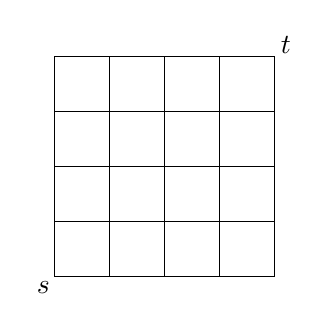
\begin{tikzpicture}[scale=0.7]
        \foreach \i in {0,...,4} {
          \draw (\i,0) -- (\i,4);
        }
        \foreach \i in {0,...,4} {
          \draw (0,\i) -- (4,\i);
        }

        \node at (-0.2, -0.2) {$s$};
        \node at (4.2, 4.2) {$t$};
      \end{tikzpicture}
    \end{figure}
  }
\end{frame}

\begin{frame}{\ctitle{Planar Graph}}
  \onslide<1-> {
    \begin{definition}
      對於平版圖 $G = (V, E)$(也就是平面圖加上一個嵌於平面的方法),$G$ 的對偶圖(Dual)定義為
      $G^{*} = (F, E^{*)})$,其中 $F$ 為 $G$ 的面,而對於所有 $E$ 中的邊 $e$,若在 $G$ 中
      $e$ 兩側的面分別為 $f_1$ 與 $f_2$,則 $(f_1, f_2) \in E^{*}$。
    \end{definition}
  }
  \onslide<2-> {
    \alt<3> {
      \begin{theorem}
        $G$ 的環空間等於 $G^{*}$ 的割空間,且 $G$ 的割空間等於 $G^{*}$ 的環空間。
      \end{theorem}
    } {
      \begin{figure}[H]
        \centering
        \begin{tikzpicture}[scale=1.5]
          \tikzset{vertex/.style = {shape=circle,draw,minimum size=1em}}
          \tikzset{edge/.style = {-,> = latex'}}
          \node[vertex] (a) at (0, 0) {};
          \node[vertex] (b) at (-1, -1) {};
          \node[vertex] (c) at (1, -1) {};
          \node[vertex] (d) at (0, -2) {};
          \node[vertex] (e) at (2.5, -1) {};

          \draw[edge] (a) to (b);
          \draw[edge] (a) to (c);
          \draw[edge] (b) to (d);
          \draw[edge] (c) to (d);
          \draw[edge] (e) to (a);
          \draw[edge] (e) to (d);
          \draw[edge] (b) to (c);
        \end{tikzpicture}
      \end{figure}
    }
  }
\end{frame}

\begin{frame}{\ctitle{Planar Max Cut}}
  \begin{problem}[Planar Max Cut]
    給定一個平面圖 $G$,找到一個點集 $S$ 使得連接 $S$ 與 $V(G) \setminus S$ 的邊數最多。

    \begin{itemize}
      \item $1 \leq n \leq 200$
      \item $1 \leq m \leq 1000$
    \end{itemize}
  \end{problem}
\end{frame}

\subsection{推廣樹 DP}

\begin{frame}{\ctitle{Tree Decomposition}}
  \begin{definition}[樹分解]
    對於圖 $G$,$G$ 的一個樹分解(Tree Decomposition)為 $(X, T)$,其中

    \begin{itemize}
      \item $X = \{X_1, X_2, \ldots, X_k\}$ 是一個 $G$ 的點集組成的序列,也就是
        $X_i \subseteq V(G)$($X_v$ 通常被稱為一個 bag)
      \item $T$ 是以 $X$ 為節點的一棵樹
    \end{itemize}

    \onslide<2-> {
      使得

      \begin{itemize}
        \item $X_1 \cup X_2 \cup \cdots \cup X_k = V(G)$,也就是 $G$ 中的每個節點都至少在
          一個 $X_i$ 中
        \item 對於所有 $G$ 中的邊 $(u, v)$,存在 $X_i$ 使得 $u$ 跟 $v$ 都在 $X_i$ 中
        \item 對於所有 $G$ 中的節點 $v$,包含 $v$ 的 $X_i$ 在 $T$ 中是一個連通子樹
      \end{itemize}
    }
  \end{definition}
\end{frame}

\begin{frame}{\ctitle{Tree Decomposition}}
  \begin{figure}[H]
    \centering
    \begin{tikzpicture}[scale=2]
      \tikzset{vertex/.style = {shape=circle,draw,minimum size=1.5em}}
      \tikzset{edge/.style = {-,> = latex'}}
      \node[vertex] (a) at (0, 0) {$1$};
      \node[vertex] (b) at (1, 0) {$2$};
      \node[vertex] (c) at (2, 0) {$3$};
      \node[vertex] (d) at (0, -1) {$4$};
      \node[vertex] (e) at (2, -1) {$5$};
      \node[vertex] (f) at (0, -2) {$6$};
      \node[vertex] (g) at (1, -2) {$7$};
      \node[vertex] (h) at (2, -2) {$8$};

      \draw[edge] (a) to (b);
      \draw[edge] (c) to (b);
      \draw[edge] (a) to (d);
      \draw[edge] (b) to (d);
      \draw[edge] (b) to (e);
      \draw[edge] (c) to (e);
      \draw[edge] (d) to (f);
      \draw[edge] (f) to (g);
      \draw[edge] (g) to (h);
      \draw[edge] (e) to (h);
      \draw[edge] (d) to (g);
      \draw[edge] (e) to (g);
      \draw[edge] (b) to (g);
    \end{tikzpicture}
  \end{figure}
\end{frame}

\begin{frame}{\ctitle{Good Tree Decomposition}}
  \begin{itemize}
    \item Introduce node $v$:
      \[ X_v = X_u \cup \{x\} \]
    \item Forget node $v$:
      \[ X_v = X_u \setminus \{x\} \]
    \item Join node $v$:
      \[ X_v = X_{u_1} = X_{u_2} \]
  \end{itemize}
\end{frame}

\begin{frame}{\ctitle{Maximum Weighted Independent Set}}
  \onslide<1-> {
    \begin{itemize}
      \item Introduce node $v$:
        \onslide<2-> {
          \[ dp(v, S) =
            \begin{cases}
              dp(u, S), & x \notin S \\
              w(x) + dp(u, S \setminus \{x\}), & \text{若 $S$ 是獨立的} \\
              -\infty, & \text{otherwise}
            \end{cases}
          \]
        }
      \item Forget node $v$:
        \onslide<3-> {
          \[
            dp(v, S) = \max(dp(u, S), dp(u, S \cup \{x\}))
          \]
        }
      \item Join node $v$:
        \onslide<4-> {
          \[
            dp(v, S) = dp(u_1, S) + dp(u_2, S) - w(S)
          \]
        }
    \end{itemize}
  }
\end{frame}

\end{document}
